\chapter{Orbital Mechanics and Elements}
\label{chap:orbital_mechanics}

\section{Introduction}

The motion of asteroids is governed by gravitational forces, primarily from the Sun but with significant perturbations from planets. As \citet{MilaniGronchi2010} state, ``asteroid orbit determination is the foundation of all predictions, including occultations.''

This chapter describes:
\begin{itemize}
    \item Classical Keplerian elements and their limitations
    \item Equinoctial elements (used by AstDyS and \ioccultcalc{})
    \item Cartesian state vectors
    \item Conversions between representations
    \item Two-body motion and Kepler's equation
\end{itemize}

\section{Classical Orbital Elements}

\subsection{Keplerian Elements}

Six elements define an orbit in the two-body problem:

\begin{figure}[htbp]
\centering
\begin{tikzpicture}[scale=1.2]
    % Reference plane (ecliptic)
    \draw[blue,dashed] (-3,0) -- (3,0);
    \draw[blue,dashed] (0,-3) -- (0,3);
    \fill[blue,opacity=0.1] (0,0) circle (2.5cm);
    \node[blue] at (3.2,0.3) {Ecliptic};
    
    % Sun at focus
    \filldraw[yellow,draw=orange,ultra thick] (0.8,0) circle (0.12) node[below=0.2cm] {Sun};
    
    % Orbit ellipse (inclined and rotated)
    \begin{scope}[canvas is xy plane at z=0,transform shape]
        \draw[red,thick,rotate=30] (0.8,0) ellipse (2cm and 1.5cm);
    \end{scope}
    
    % Perihelion
    \filldraw[purple] (2.5,0.8) circle (0.05) node[right] {Perihelion};
    \draw[->,purple,thick] (0.8,0) -- (2.5,0.8) node[midway,above] {$a(1-e)$};
    
    % Asteroid position
    \filldraw[brown] (1.2,2.3) circle (0.06) node[above right] {Asteroid};
    
    % Ascending node
    \filldraw[green!60!black] (1.8,0) circle (0.05) node[below] {$\Omega$ (Asc. Node)};
    \draw[->,green!60!black,thick] (0,0) -- (1.8,0);
    
    % Inclination
    \draw[->,cyan,thick] (0,0) -- (0,2) node[above] {$Z$ (ENP)};
    \draw[cyan,thick] (1,0) arc (0:30:1);
    \node[cyan] at (1.3,0.3) {$i$};
    
    % Argument of perihelion
    \draw[purple,thick] (1.8,0) arc (-10:20:1.2);
    \node[purple] at (2.2,0.5) {$\omega$};
    
    % Longitude of ascending node
    \draw[green!60!black,thick] (1.5,0) arc (0:30:1.5);
    
    % True anomaly
    \draw[brown,thick] (2.3,0.7) arc (10:60:0.8);
    \node[brown] at (2.0,1.2) {$\nu$};
    
    % Vernal equinox
    \draw[->,black,ultra thick] (0,0) -- (3,0) node[right] {$\gamma$};
\end{tikzpicture}
\caption{Classical orbital elements. The orbit is defined by: semi-major axis $a$, eccentricity $e$, inclination $i$, longitude of ascending node $\Omega$, argument of perihelion $\omega$, and true anomaly $\nu$ (or mean anomaly $M$). ENP = Ecliptic North Pole.}
\label{fig:orbital_elements}
\end{figure}

\begin{description}
    \item[$a$] \textbf{Semi-major axis} (AU): size of orbit, $a = (r_{\text{max}} + r_{\text{min}})/2$
    \item[$e$] \textbf{Eccentricity} (dimensionless): shape, $e = (r_{\text{max}} - r_{\text{min}})/(r_{\text{max}} + r_{\text{min}})$
        \begin{itemize}
            \item $e = 0$: circular orbit
            \item $0 < e < 1$: ellipse (all asteroids)
            \item $e = 1$: parabola (some comets)
            \item $e > 1$: hyperbola (interstellar objects)
        \end{itemize}
    \item[$i$] \textbf{Inclination} (degrees): angle from reference plane (ecliptic), $0° \leq i \leq 180°$
    \item[$\Omega$] \textbf{Longitude of ascending node} (degrees): where orbit crosses ecliptic northward, $0° \leq \Omega < 360°$
    \item[$\omega$] \textbf{Argument of perihelion} (degrees): angle from node to perihelion, $0° \leq \omega < 360°$
    \item[$M$] \textbf{Mean anomaly} (degrees): uniform angular motion, $M = n(t - t_0)$ where $n = \sqrt{\mu/a^3}$
\end{description}

\textbf{Alternative to $M$:}
\begin{itemize}
    \item $\nu$ = true anomaly (actual angle from perihelion)
    \item $E$ = eccentric anomaly (geometric construction)
    \item $t_p$ = time of perihelion passage
\end{itemize}

\subsection{Singularities in Classical Elements}

Classical elements have \textbf{singularities}:

\begin{table}[htbp]
\centering
\caption{Singularities in classical orbital elements}
\label{tab:classical_singularities}
\begin{tabular}{lcp{7cm}}
\hline
\textbf{Condition} & \textbf{Problem} & \textbf{Physical Meaning} \\
\hline
$e \rightarrow 0$ & $\omega$ undefined & Circular orbit: no perihelion \\
$i \rightarrow 0°$ & $\Omega$ undefined & Equatorial orbit: no node \\
$i \rightarrow 180°$ & $\Omega$ undefined & Retrograde equatorial \\
$e \rightarrow 0$, $i \rightarrow 0$ & $\omega$, $\Omega$, $M$ all ill-defined & Circular equatorial \\
\hline
\end{tabular}
\end{table}

These singularities cause:
\begin{itemize}
    \item Numerical instability in orbit propagation
    \item Large derivatives near singular points
    \item Poor performance in orbit determination
    \item Ambiguity in initial conditions
\end{itemize}

\textbf{Solution:} Use non-singular element sets like \textbf{equinoctial elements}.

\section{Equinoctial Orbital Elements}

\subsection{Definition}

Equinoctial elements avoid singularities for small $e$ and $i$ \citep{BrouckeBat1980,Broucke1969}:

\begin{align}
a &= \text{semi-major axis (same as classical)} \label{eq:equi_a} \\
h &= e \sin(\omega + \Omega) \label{eq:equi_h} \\
k &= e \cos(\omega + \Omega) \label{eq:equi_k} \\
p &= \tan(i/2) \sin\Omega \label{eq:equi_p} \\
q &= \tan(i/2) \cos\Omega \label{eq:equi_q} \\
\lambda &= M + \omega + \Omega \quad \text{(mean longitude)} \label{eq:equi_lambda}
\end{align}

\textbf{Properties:}
\begin{itemize}
    \item \textbf{Non-singular} for $e < 1$, $0° \leq i < 180°$ (all asteroidal orbits)
    \item \textbf{Used by AstDyS:} asteroid database provides $(a, h, k, p, q, \lambda)$
    \item \textbf{Smooth derivatives:} suitable for numerical integration and least squares
    \item \textbf{Physical interpretation:}
        \begin{itemize}
            \item $(h, k)$: eccentricity vector components
            \item $(p, q)$: inclination vector components (half-tangent)
            \item $\lambda$: mean longitude (combines $M$, $\omega$, $\Omega$)
        \end{itemize}
\end{itemize}

\subsection{Geometric Interpretation}

\begin{figure}[htbp]
\centering
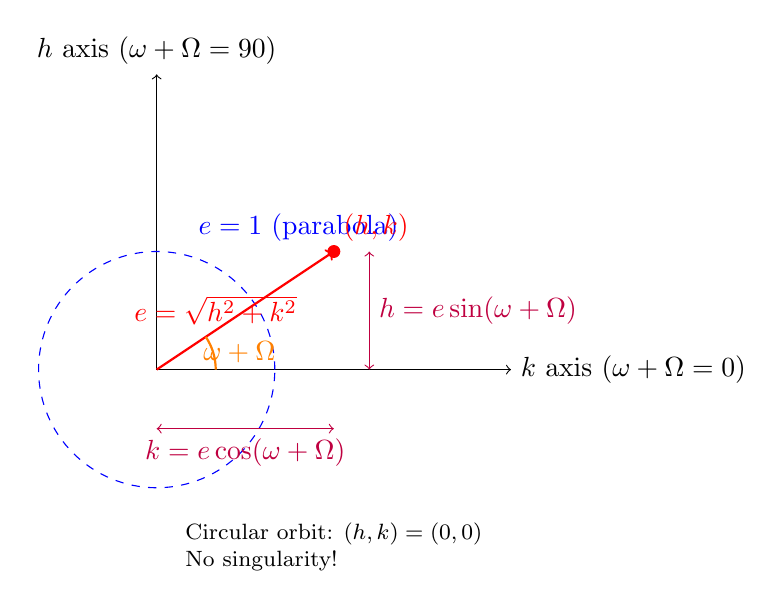
\begin{tikzpicture}[scale=1.5]
    % Eccentricity vector (h,k)
    \draw[->] (0,0) -- (3,0) node[right] {$k$ axis ($\omega+\Omega=0°$)};
    \draw[->] (0,0) -- (0,2.5) node[above] {$h$ axis ($\omega+\Omega=90°$)};
    
    \draw[blue,dashed] (0,0) circle (1cm);
    \node[blue] at (1.2,1.2) {$e=1$ (parabola)};
    
    % Example asteroid
    \filldraw[red] (1.5,1.0) circle (0.05) node[above right] {$(h, k)$};
    \draw[->,red,thick] (0,0) -- (1.5,1.0);
    
    % Eccentricity
    \draw[<->,purple] (0,-0.5) -- (1.5,-0.5) node[midway,below] {$k = e\cos(\omega+\Omega)$};
    \draw[<->,purple] (1.8,0) -- (1.8,1.0) node[midway,right] {$h = e\sin(\omega+\Omega)$};
    
    % Magnitude
    \node[red] at (0.5,0.5) {$e = \sqrt{h^2+k^2}$};
    
    % Angle
    \draw[orange,thick] (0.5,0) arc (0:33.7:0.5);
    \node[orange] at (0.7,0.15) {$\omega+\Omega$};
    
    \node[align=left,font=\footnotesize] at (1.5,-1.5) {
        Circular orbit: $(h,k) = (0,0)$ \\
        No singularity!
    };
\end{tikzpicture}
\caption{Equinoctial eccentricity vector $(h, k)$. The magnitude $\sqrt{h^2 + k^2} = e$ gives eccentricity, and the angle $\arctan(h/k) = \omega + \Omega$ gives perihelion direction. Unlike classical elements, $(h, k) = (0, 0)$ for circular orbits is well-defined.}
\label{fig:equinoctial_hk}
\end{figure}

\subsection{Conversion: Equinoctial $\leftrightarrow$ Classical}

\textbf{Equinoctial to classical:}
\begin{align}
a &= a \label{eq:equi_to_class_a} \\
e &= \sqrt{h^2 + k^2} \label{eq:equi_to_class_e} \\
i &= 2 \arctan\sqrt{p^2 + q^2} \label{eq:equi_to_class_i} \\
\Omega &= \arctan(p, q) = \arctan2(p, q) \label{eq:equi_to_class_Omega} \\
\omega &= \arctan(h, k) - \Omega \label{eq:equi_to_class_omega} \\
M &= \lambda - \omega - \Omega \label{eq:equi_to_class_M}
\end{align}

\textbf{Special cases:}
\begin{itemize}
    \item If $e = 0$: set $\omega = 0$ (arbitrary, orbit is circular)
    \item If $i = 0$: set $\Omega = 0$ (arbitrary, orbit is equatorial)
    \item Use \texttt{atan2(y, x)} to handle all quadrants correctly
\end{itemize}

\textbf{Classical to equinoctial:} Use Equations~\ref{eq:equi_h}--\ref{eq:equi_lambda}.

\subsection{Example Conversion}

\textbf{Asteroid (472) Roma from AstDyS:}
\begin{align*}
a &= 2.534 \text{ AU} \\
h &= +0.0821 \\
k &= +0.1234 \\
p &= +0.0453 \\
q &= -0.0123 \\
\lambda &= 123.456° \quad \text{(at epoch JD 2460000.5)}
\end{align*}

\textbf{Convert to classical:}
\begin{align*}
e &= \sqrt{0.0821^2 + 0.1234^2} = 0.1482 \\
i &= 2\arctan\sqrt{0.0453^2 + 0.0123^2} = 2 \arctan(0.0469) = 5.38° \\
\Omega &= \arctan2(0.0453, -0.0123) = 105.2° \\
\omega + \Omega &= \arctan2(0.0821, 0.1234) = 33.6° \\
\omega &= 33.6° - 105.2° = -71.6° = 288.4° \\
M &= 123.456° - 288.4° - 105.2° = -270.1° = 89.9°
\end{align*}

\section{Cartesian State Vectors}

\subsection{Position and Velocity}

The complete orbital state is given by position $\vect{r}$ and velocity $\vect{v}$:

\begin{equation}
\vect{X} = (\vect{r}, \vect{v}) = (x, y, z, \dot{x}, \dot{y}, \dot{z})
\label{eq:state_vector}
\end{equation}

in some reference frame (typically heliocentric ecliptic J2000).

\textbf{Advantages:}
\begin{itemize}
    \item No singularities (well-defined for all orbits)
    \item Direct use in numerical integration
    \item Simple Newtonian equations of motion: $\ddot{\vect{r}} = -\frac{\mu}{r^3}\vect{r} + \vect{a}_{\text{pert}}$
\end{itemize}

\textbf{Disadvantages:}
\begin{itemize}
    \item 6 numbers vs. 6 orbital elements (no reduction in dimensionality)
    \item Less intuitive (hard to visualize orbit from Cartesian state)
    \item Larger numerical values (positions in km, velocities in km/s)
\end{itemize}

\subsection{Conversion: Elements $\rightarrow$ Cartesian}

\begin{algorithm}[H]
\caption{Orbital Elements to Cartesian State Vector}
\label{alg:elements_to_cartesian}
\begin{algorithmic}[1]
\REQUIRE Elements $(a, e, i, \Omega, \omega, M)$ or $(a, h, k, p, q, \lambda)$, epoch $t$
\STATE Compute true anomaly $\nu$ from mean anomaly $M$ (Kepler's equation, Sec.~\ref{sec:kepler})
\STATE Compute distance: $r = \frac{a(1-e^2)}{1 + e\cos\nu}$
\STATE \textbf{Orbital plane coordinates:}
\STATE $x_{\text{orb}} = r \cos\nu$, \quad $y_{\text{orb}} = r \sin\nu$
\STATE $\dot{x}_{\text{orb}} = -\sqrt{\mu/p} \sin\nu$, \quad $\dot{y}_{\text{orb}} = \sqrt{\mu/p} (e + \cos\nu)$
\STATE where $p = a(1-e^2)$ is semi-latus rectum, $\mu = GM_{\odot}$
\STATE \textbf{Rotation to reference frame:}
\STATE $\mat{R} = \mat{R}_z(-\Omega) \cdot \mat{R}_x(-i) \cdot \mat{R}_z(-\omega)$
\STATE $\vect{r} = \mat{R} \cdot (x_{\text{orb}}, y_{\text{orb}}, 0)^T$
\STATE $\vect{v} = \mat{R} \cdot (\dot{x}_{\text{orb}}, \dot{y}_{\text{orb}}, 0)^T$
\RETURN $\vect{X} = (\vect{r}, \vect{v})$
\end{algorithmic}
\end{algorithm}

\subsection{Conversion: Cartesian $\rightarrow$ Elements}

This requires computing:
\begin{enumerate}
    \item Specific angular momentum: $\vect{h} = \vect{r} \times \vect{v}$
    \item Eccentricity vector: $\vect{e} = \frac{\vect{v} \times \vect{h}}{\mu} - \frac{\vect{r}}{r}$
    \item Node vector: $\vect{n} = \hat{z} \times \vect{h}$
\end{enumerate}

Then:
\begin{align}
a &= \frac{1}{2/r - v^2/\mu} \label{eq:cart_to_a} \\
e &= |\vect{e}| \label{eq:cart_to_e} \\
i &= \arccos(h_z / |\vect{h}|) \label{eq:cart_to_i} \\
\Omega &= \arctan2(n_y, n_x) \label{eq:cart_to_Omega} \\
\omega &= \arctan2(e_z / \sin i, e_x \cos\Omega + e_y \sin\Omega) \label{eq:cart_to_omega} \\
\nu &= \arctan2(\vect{r} \cdot \vect{v} / |\vect{h}|, 1 - r/p) \label{eq:cart_to_nu}
\end{align}

\section{Two-Body Motion}

\subsection{Kepler's Laws}

\textbf{First Law:} Orbits are ellipses with the Sun at one focus.

\textbf{Second Law:} A line from the Sun to the planet sweeps equal areas in equal times (conservation of angular momentum).

\begin{equation}
\frac{dA}{dt} = \frac{1}{2}|\vect{r} \times \vect{v}| = \frac{|\vect{h}|}{2} = \text{constant}
\end{equation}

\textbf{Third Law:} The square of the orbital period is proportional to the cube of the semi-major axis.

\begin{equation}
T^2 = \frac{4\pi^2}{\mu} a^3
\label{eq:kepler_third}
\end{equation}

For $\mu = GM_{\odot} = 1.32712440018 \times 10^{20}$ m$^3$/s$^2$ and $a$ in AU, $T$ in years:
\begin{equation}
T = a^{3/2} \quad \text{(Kepler's third law simplified)}
\end{equation}

\textbf{Example:} (472) Roma with $a = 2.534$ AU:
\begin{equation}
T = 2.534^{1.5} = 4.04 \text{ years} = 1475 \text{ days}
\end{equation}

\subsection{Kepler's Equation}
\label{sec:kepler}

The relationship between mean anomaly $M$ (uniform in time) and true anomaly $\nu$ (actual angle) is:

\begin{align}
M &= E - e\sin E \quad \text{(Kepler's equation)} \label{eq:kepler} \\
\nu &= 2\arctan\left(\sqrt{\frac{1+e}{1-e}} \tan\frac{E}{2}\right) \label{eq:eccentric_to_true}
\end{align}

where $E$ is the eccentric anomaly.

\textbf{Problem:} Equation~\ref{eq:kepler} is transcendental—no closed-form solution for $E$ given $M$ and $e$.

\subsection{Solving Kepler's Equation}

\textbf{Newton-Raphson iteration:}

\begin{algorithm}[H]
\caption{Kepler's Equation via Newton-Raphson}
\label{alg:kepler_newton}
\begin{algorithmic}[1]
\REQUIRE Mean anomaly $M$, eccentricity $e$, tolerance $\epsilon = 10^{-12}$
\STATE $E \leftarrow M$ \quad // Initial guess
\FOR{$i = 1$ to $10$} \quad // Usually converges in 3--5 iterations
    \STATE $f \leftarrow E - e\sin E - M$
    \STATE $f' \leftarrow 1 - e\cos E$
    \STATE $\Delta E \leftarrow -f / f'$
    \STATE $E \leftarrow E + \Delta E$
    \IF{$|\Delta E| < \epsilon$}
        \STATE \textbf{break}
    \ENDIF
\ENDFOR
\RETURN $E$
\end{algorithmic}
\end{algorithm}

\textbf{Convergence:} Quadratic for $e < 0.8$. For high eccentricity ($e > 0.9$), use Laguerre's method or continued fractions.

\textbf{Example:} $M = 89.9°$, $e = 0.1482$
\begin{align*}
E_0 &= 89.9° = 1.5690 \text{ rad} \\
f_0 &= 1.5690 - 0.1482 \sin(1.5690) - 1.5690 = -0.1482 \\
E_1 &= 1.5690 - (-0.1482)/(1 - 0.1482\cos 1.5690) = 1.7172 \text{ rad} \\
E_2 &= 1.7039 \text{ rad (converged to } 10^{-6}\text{)}
\end{align*}

Then:
\begin{equation}
\nu = 2\arctan\left(\sqrt{\frac{1.1482}{0.8518}} \tan\frac{1.7039}{2}\right) = 101.3°
\end{equation}

\begin{figure}[htbp]
\centering
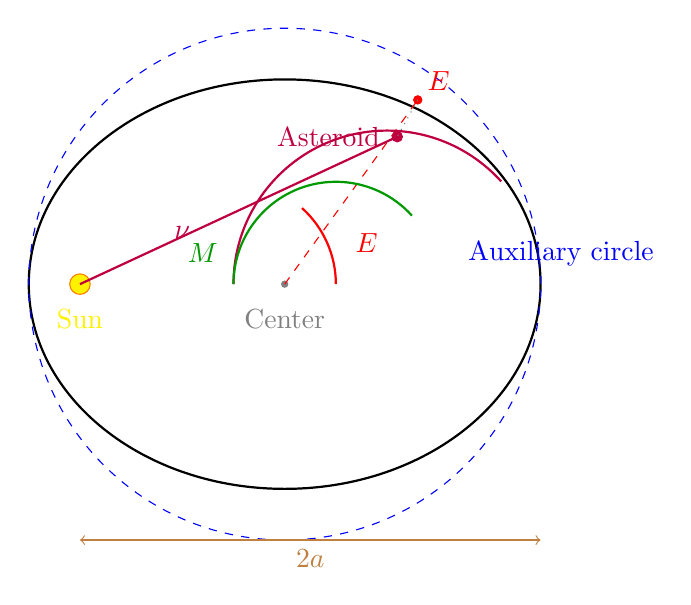
\begin{tikzpicture}[scale=1.3]
    % Ellipse
    \draw[thick] (0.5,0) ellipse (2.5cm and 2cm);
    
    % Sun at focus
    \filldraw[yellow,draw=orange] (-1.5,0) circle (0.1) node[below=0.2cm] {Sun};
    
    % Center
    \filldraw[gray] (0.5,0) circle (0.03) node[below=0.2cm] {Center};
    
    % Auxiliary circle
    \draw[blue,dashed] (0.5,0) circle (2.5cm);
    \node[blue] at (3.2,0.3) {Auxiliary circle};
    
    % Eccentric anomaly point
    \draw[red,dashed] (0.5,0) -- (1.8,1.8) node[above right] {$E$};
    \filldraw[red] (1.8,1.8) circle (0.04);
    
    % True anomaly (actual asteroid)
    \draw[purple,thick] (-1.5,0) -- (1.6,1.44);
    \filldraw[purple] (1.6,1.44) circle (0.05) node[left=0.1cm] {Asteroid};
    \draw[purple,thick] (0,0) arc (180:42:1.5);
    \node[purple] at (-0.5,0.5) {$\nu$};
    
    % Mean anomaly (uniform motion)
    \draw[green!60!black,thick] (0,0) arc (180:42:1);
    \node[green!60!black] at (-0.3,0.3) {$M$};
    
    % Eccentric anomaly
    \draw[red,thick] (1,0) arc (0:48:1);
    \node[red] at (1.3,0.4) {$E$};
    
    % Projection
    \draw[gray,dotted] (1.8,1.8) -- (1.6,1.44);
    
    % Semi-major axis
    \draw[<->,brown] (-1.5,-2.5) -- (3,-2.5) node[midway,below] {$2a$};
\end{tikzpicture}
\caption{Relationship between mean anomaly $M$ (green, uniform angular motion), eccentric anomaly $E$ (red, on auxiliary circle), and true anomaly $\nu$ (purple, actual position). Kepler's equation $M = E - e\sin E$ connects them.}
\label{fig:kepler_anomalies}
\end{figure}

\section{Orbital Energy and Period}

\subsection{Specific Orbital Energy}

The total energy per unit mass:

\begin{equation}
\mathcal{E} = \frac{v^2}{2} - \frac{\mu}{r} = -\frac{\mu}{2a}
\label{eq:orbital_energy}
\end{equation}

\textbf{Key insight:} Energy depends only on $a$, not on $e$ or $i$.

\begin{itemize}
    \item $\mathcal{E} < 0$: bound orbit (ellipse)
    \item $\mathcal{E} = 0$: parabolic escape
    \item $\mathcal{E} > 0$: hyperbolic escape
\end{itemize}

\subsection{Orbital Period}

From Kepler's third law (Eq.~\ref{eq:kepler_third}):

\begin{equation}
T = 2\pi\sqrt{\frac{a^3}{\mu}}
\end{equation}

In convenient units (AU and days):
\begin{equation}
T[\text{days}] = 365.25 \times a[\text{AU}]^{3/2}
\end{equation}

\textbf{Mean motion:}
\begin{equation}
n = \frac{2\pi}{T} = \sqrt{\frac{\mu}{a^3}} \quad \text{(rad/s or deg/day)}
\end{equation}

For (472) Roma ($a = 2.534$ AU):
\begin{equation}
n = \frac{360°}{1475 \text{ days}} = 0.244°/\text{day}
\end{equation}

\section{Perturbations Preview}

Two-body motion is an \textbf{approximation}. Real asteroids experience:

\begin{enumerate}
    \item \textbf{Planetary perturbations:} Jupiter's gravity ($\Delta a/a \sim 10^{-5}$)
    \item \textbf{Non-spherical Sun:} Oblateness ($J_2 \sim 10^{-7}$, negligible)
    \item \textbf{Relativistic effects:} Perihelion precession ($\sim 5''/century$ for Mercury)
    \item \textbf{Radiation pressure:} Yarkovsky effect (secular $\Delta a$)
    \item \textbf{Close encounters:} Sudden orbit changes
\end{enumerate}

These are treated in Chapter~\ref{chap:perturbations}.

\section{Summary}

This chapter established orbital mechanics foundations:

\begin{itemize}
    \item \textbf{Classical elements:} $(a, e, i, \Omega, \omega, M)$ — intuitive but singular for $e=0$, $i=0$
    \item \textbf{Equinoctial elements:} $(a, h, k, p, q, \lambda)$ — non-singular, used by AstDyS
    \item \textbf{Cartesian state:} $(\vect{r}, \vect{v})$ — universal, no singularities
    \item \textbf{Kepler's equation:} $M = E - e\sin E$ solved by Newton-Raphson
    \item \textbf{Two-body motion:} Foundation for perturbation theory
\end{itemize}

Figures~\ref{fig:orbital_elements}, \ref{fig:equinoctial_hk}, and \ref{fig:kepler_anomalies} illustrate the element definitions and anomaly relationships. Table~\ref{tab:classical_singularities} quantifies singularity issues.

\textbf{Key relationships:}
\begin{align*}
e &= \sqrt{h^2 + k^2} \quad \text{(equinoctial)} \\
T &= 365.25 \times a^{3/2} \text{ days} \quad \text{(period)} \\
M &= E - e\sin E \quad \text{(Kepler's equation)}
\end{align*}

\textbf{For \ioccultcalc{}:}
\begin{itemize}
    \item Import equinoctial elements from AstDyS (no conversion singularities)
    \item Convert to Cartesian for numerical integration (Chapter~\ref{chap:integration})
    \item Use Keplerian two-body for fast predictions (error $\sim$10 km/year)
    \item Use full perturbations for high precision (Chapter~\ref{chap:perturbations})
\end{itemize}

\textbf{References:}
\begin{itemize}
    \item Milani \& Gronchi (2010) \citep{MilaniGronchi2010}: comprehensive orbit determination
    \item Broucke \& Cefola (1972) \citep{BrouckeBat1980}: equinoctial elements
    \item Vallado (2013) \citep{Vallado2013}: practical orbital mechanics
    \item Danby (1988) \citep{Danby1988}: Kepler equation solvers
\end{itemize}

Next chapter: Numerical Integration Methods.
